%!TEX root = ../AutF3.tex
% -- Author: Phil Steinhorst, p.st@wwu.de
\chapter{Gruppenwirkungen auf kubischen Komplexen}
\label{cha:wirkungen_kubische_komplexe}
	In diesem Kapitel wollen wir zeigen, dass endlich erzeugte Gruppen, die Kazhdans Eigenschaft $\prT$ innehaben, eine weitere Fixpunkteigenschaft besitzen. Dazu betrachten wir kubische Komplexe und anschließend isometrische Wirkungen von Gruppen auf diesen. Abgeschlossen wird dieses Kapitel durch eine Einführung der Eigenschaften $\prFC$ und $\prFA$, die die Eigenschaft $\prT$ impliziert.
	
\section{Eine Einführung in kubische Komplexe}
\label{sec:kub_kpx}
	Wir beginnen mit einer Einführung des Begriffs des kubischen Komplexes. Dabei richten wir uns im Wesentlichen nach den Ausführung in \cite[S. 7\psqq]{Schwer}.

\begin{definition}[Würfel, Seite]
	Eine \textbf{Seite} des $n$-Würfels $C=[0,1]^n \subseteq \RR^n, n \geq 1$, ist eine Teilmenge $F \subseteq C$ gegeben durch
	\[ F = F_1 \times F_2 \times \dots \times F_n \text{ mit } F_i \in \{ \{0\}, \{1\}, [0,1]\}.\]
	Die auf $C$ eingeschränkte euklidische Metrik des $\RR^n$ bezeichnen wir mit $d_C$. Den $0$-Würfel definieren wir als $[0,1]^0 := \{0\}$. Wir nennen $\dim(C) := n$ die \textbf{Dimension} von $C$. Offensichtlich sind nichtleere Schnitte von Seiten ebenfalls eine Seite von $C$.
\end{definition}

\begin{definition}[Kubischer Komplex]
	Seien $C, C'$ zwei Würfel mit zugehörigen Seiten $F \subseteq C, F' \subseteq C'$. Eine bijektive Isometrie $\varphi\colon F \rightarrow F'$ heißt \textbf{Klebung} von $C$ und $C'$.
	
	Sei $\mathcal{C}$ eine Familie von Würfeln (i. A. verschiedener Dimensionen) und $\mathcal{S}$ eine Familie von Klebungen von Würfeln in $\mathcal{C}$ mit folgenden Eigenschaften:
	\begin{enumerate}[(i)]
		\item Kein Würfel ist mit sich selbst verklebt.
		\item Je zwei Würfel aus $\mathcal{C}$ sind höchstens einmal miteinander verklebt.
	\end{enumerate}
	
	Sei $\sim$ die durch
	\[ x \sim y :\Leftrightarrow \text{ es existiert ein } \varphi \in \mathcal{S} \text{ mit } x \in \dom(\varphi) \text{ und } \varphi(x) = y \]
	erzeugte Äquivalenzrelation	auf der disjunkten Vereinigung $\sqcup_{C \in \mathcal{C}} C$. Dann definieren $\mathcal{C}$ und $\mathcal{S}$ den \textbf{kubischen Komplex} $X$ durch
	\[ X := \enbrace*{\bigsqcup_{C \in \mathcal{C}} C} \diagup \sim. \]	
\end{definition}

\begin{figure}[h]
	\centering
	$\vcenter{\hbox{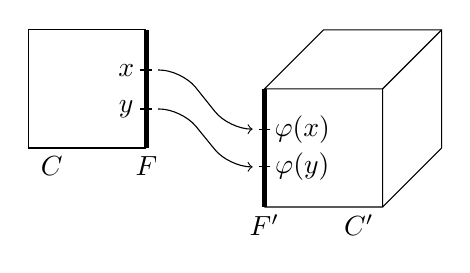
\begin{tikzpicture}[scale=1.5]
	\draw (1,0) -- (0,0) -- (0,1) -- (1,1);
	\draw [ultra thick] (1,0) -- (1,1);
	\draw (0.2,-.15) node {$C$};
	\draw (1,-.15) node {$F$};
	
	\draw (.95,0.33) -- (1.05,0.33) node[pos=-1.2] {$y$};
	\draw (.95,0.66) -- (1.05,0.66) node[pos=-1.2] {$x$};
	
	\draw (2,-.5) -- (3,-.5) -- (3,.5) -- (2,.5) -- (2.5,1) -- (3.5,1) -- (3.5,0) -- (3,-.5);
	\draw (3,.5) -- (3.5,1);
	\draw [ultra thick] (2,.5) -- (2,-.5);
	\draw (2,-.65) node {$F'$};
	\draw (2.8,-.65) node {$C'$};
	
	\draw (1.95,.16) -- (2.05,.16) node [pos=3.7] {$\varphi(x)$};
	\draw (1.95,-.16) -- (2.05,-.16) node [pos=3.7] {$\varphi(y)$};	
	
	\draw [->, rounded corners=8pt] (1.1,.66) -- (1.3,.66) -- (1.7,.16) -- (1.9,.16);
	\draw [->, rounded corners=8pt] (1.1,.33) -- (1.3,.33) -- (1.7,-.16) -- (1.9,-.16);
	\end{tikzpicture}
	\hspace{1cm}}}
	\rightsquigarrow
	\vcenter{\hbox{\hspace{1cm}
	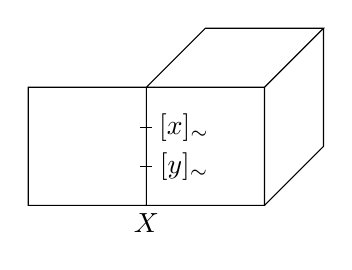
\begin{tikzpicture}[scale=1.5]
	\draw (2,1) -- (0,1) -- (0,0) -- (1,0) -- (1,1) -- (1.5,1.5) -- (2.5,1.5) -- (2,1) -- (2,0) -- (1,0);
	\draw (2,0) -- (2.5,.5) -- (2.5,1.5);
	\draw (1,-.15) node {$X$};
	\draw (.95,.33) -- (1.05,.33) node[pos=3.7] {$[y]_\sim$};
	\draw (.95,.66) -- (1.05,.66) node[pos=3.7] {$[x]_\sim$};
	\end{tikzpicture}
	}}$
	\caption{Konstruktion eines kubischen Komplexes durch Verklebung zweier Würfel.}
\end{figure}

\begin{beispiel}
	\mbox{} \\[-1.4cm]
	\begin{itemize}
		\item Simpliziale Bäume sind kubische Komplexe bestehend aus $0$- und $1$-Würfeln.
		\item $\RR^n$ lässt sich auf kanonische Weise mit Einheitswürfeln $C_i \simeq [0,1]^n$ überdecken und kann daher als kubischer Komplex aufgefasst werden.
		\item Der Torus ist ebenfalls als kubischer Komplex auffassbar.
	\end{itemize}
\end{beispiel}

\begin{figure}[h]
	\centering
	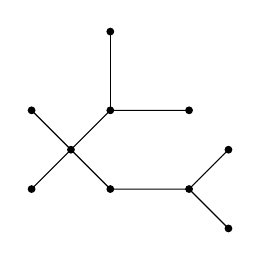
\begin{tikzpicture}[scale=1]
		\draw (0,0) -- (.5,.5) -- (1,0) -- (2,0) -- (2.5,-.5);
		\draw (2,0) -- (2.5,.5);
		\draw (0,1) -- (.5,.5) -- (1,1) -- (2,1);
		\draw (1,1) -- (1,2);
		\draw (0,0) node[fill,circle,inner sep=1pt]{};
		\draw (.5,.5) node[fill,circle,inner sep=1pt]{};
		\draw (0,1) node[fill,circle,inner sep=1pt]{};
		\draw (1,1) node[fill,circle,inner sep=1pt]{};
		\draw (1,2) node[fill,circle,inner sep=1pt]{};
		\draw (2,1) node[fill,circle,inner sep=1pt]{};
		\draw (1,0) node[fill,circle,inner sep=1pt]{};
		\draw (2,0) node[fill,circle,inner sep=1pt]{};
		\draw (2.5,-.5) node[fill,circle,inner sep=1pt]{};
		\draw (2.5,.5) node[fill,circle,inner sep=1pt]{};
	\end{tikzpicture} \hspace{2cm}
	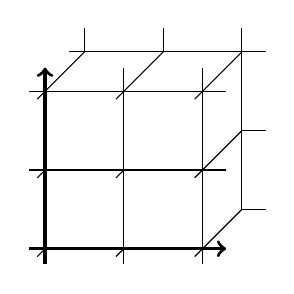
\begin{tikzpicture}[scale=1]
		\draw[->,very thick] (-.2,0) -- (2.3,0);
		\draw (-.2,1) -- (2.3,1); 
		\draw (-.2,2) -- (2.3,2); 
		\draw (.3,2.5) -- (2.8,2.5);
		
		\draw[->,very thick] (0,-.2) -- (0,2.3);
		\draw (1,-.2) -- (1,2.3);
		\draw (2,-.2) -- (2,2.3);
		\draw (2.5,.5) -- (2.5,2.8);
		
		\draw (-.1,1.9) -- (.5,2.5);
		\draw (.9,1.9) -- (1.5,2.5);
		\draw (1.9,1.9) -- (2.5,2.5);
		\draw (1.9,.9) -- (2.5,1.5);
		\draw (1.9,-.1) -- (2.5,.5);
		
		\draw (.5,2.5) -- (.5,2.8);
		\draw (1.5,2.5) -- (1.5,2.8);
		\draw (2.5,.5) -- (2.8,.5);
		\draw (2.5,1.5) -- (2.8,1.5);
		
		\draw (0,0) -- (-.1,-.1);
		\draw (1,0) -- (.9,-.1);
		\draw (0,1) -- (-.1,.9);
		\draw (1,1) -- (.9,.9);
	\end{tikzpicture} \hspace{2cm}
	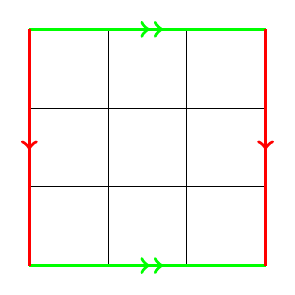
\begin{tikzpicture}[scale=1]
		\draw (0,1) -- (3,1);
		\draw (0,2) -- (3,2);
		\draw (1,0) -- (1,3);
		\draw (2,0) -- (2,3);
		
		\draw[color=green,very thick] (0,3) -- (3,3);
		\draw[->,color=green,very thick] (0,3) -- (1.7,3);
		\draw[->,color=green,very thick] (0,3) -- (1.53,3);
		\draw[color=green,very thick] (0,0) -- (3,0);
		\draw[->,color=green,very thick] (0,0) -- (1.7,0);
		\draw[->,color=green,very thick] (0,0) -- (1.53,0);
		
		\draw[color=red,very thick] (0,3) -- (0,0);
		\draw[->,color=red,very thick] (0,3) -- (0,1.47);
		\draw[color=red,very thick] (3,3) -- (3,0);
		\draw[->,color=red,very thick] (3,3) -- (3,1.47);
	\end{tikzpicture}
	\caption{Beispiele für kubische Komplexe.}
\end{figure}

Ein kubischer Komplex $X$ besitzt auf natürliche Weise zwei Metriken: Für zwei Punkte $x,y \in X$ nennen wir eine endliche Folge $\sigma = (x_0,\dots,x_m)$ von Punkten $x_i \in X$ mit $x_0 = x, x_m = y$ einen \textbf{Weg} von $x$ nach $y$, wenn für alle $i$ mit $0 \leq i \leq m-1$ ein Würfel $C_i$ von $X$ existiert mit $x_i, x_{i+1} \in C_i$. 

Die Länge des Weges definieren wir als
\[ \ell(\sigma) := \sum\limits_{i=0}^{m-1} d_{C_i} (x_i,x_{i+1}) \]
Finden wir für je zwei Punkte $x,y \in X$ stets einen solchen Weg, nennen wir $X$ \textbf{wegzusammenhängend}. In diesem Fall können wir $X$ mit der \textbf{Längenmetrik} versehen:
	\begin{equation}
	\begin{aligned}
	d_\ell \colon X \times X &\longrightarrow \RR \\
	(x,y) &\longmapsto \inf\{ \ell(\sigma) : \sigma \text{ ist Weg von } x \text{ nach } y \text{ in } X\}
	\end{aligned}
	\end{equation}
Wir betrachten im Folgenden ausschließlich wegzusammenhängende, $\cat$ vollständige kubische Komplexe, das heißt kubische Komplexe, für die der metrische Raum $(X,d_\ell)$ $\cat$ und vollständig ist.

\begin{figure}[h]
	\centering
	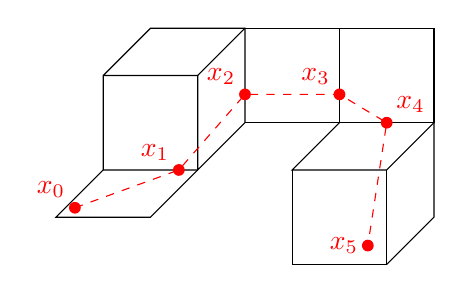
\begin{tikzpicture}[scale=1.2]
	\draw (1,0) -- (1,1) -- (0,1) -- (0,0) -- (1,0) -- (1.5,.5) -- (1.5,1.5) -- (.5,1.5) -- (0,1);
	\draw (1,1) -- (1.5,1.5);
	
	\draw (0,0) -- (-.5,-.5) -- (.5,-.5) -- (1,0);
	\draw (1.5,.5) -- (2.5,.5) -- (2.5,1.5) -- (1.5,1.5);
	\draw (2.5,1.5) -- (3.5,1.5) -- (3.5,.5) -- (2.5,.5);
	\draw (3.5,.5) -- (3,0) -- (2,0) -- (2.5,.5);
	\draw (2,0) -- (2,-1) -- (3,-1) -- (3,0);
	\draw (3,-1) -- (3.5,-.5) -- (3.5,.5);
	
	\draw [dashed, color=red] (-.3,-.4) node[fill,circle,inner sep=1.5pt]{} 
	-- (.8,0) node[fill,circle,inner sep=1.5pt]{} 
	-- (1.5,.8) node[fill,circle,inner sep=1.5pt]{} 
	-- (2.5,.8) node[fill,circle,inner sep=1.5pt]{} 
	-- (3,.5) node[fill,circle,inner sep=1.5pt]{} 
	-- (2.8,-.8) node[fill,circle,inner sep=1.5pt]{};
	
	\draw[color=red] (-.3,-.4) node[anchor = south east]{$x_0$};
	\draw[color=red] (.8,0) node[anchor = south east]{$x_1$};
	\draw[color=red] (1.5,.8) node[anchor = south east]{$x_2$};
	\draw[color=red] (2.5,.8) node[anchor = south east]{$x_3$};
	\draw[color=red] (3,.5) node[anchor = south west]{$x_4$};
	\draw[color=red] (2.8,-.8) node[anchor = east]{$x_5$};
	\end{tikzpicture}
	\caption{Ein Weg von $x_0$ nach $x_5$.} 
\end{figure}

Für dei zweite Metrik eines kubischen Komplexes $(X,d_\ell)$ betrachten wir das $1$-Skelett $X^{(1)}$, bestehend aus den Ecken und Kanten der einzelnen Würfel von $X$ (das heißt aus den Seiten der Dimension $0$ und $1$), sowie das $0$-Skelett $X^{(0)}$, welches aus den Eckpunkten der Würfel besteht. $X^{(1)}$ kann selbst als kubischer Komplex der Dimension $1$ aufgefasst werden. Die \textbf{simpliziale Metrik} von $X$ ist dann gegeben durch:
\begin{equation}
\begin{aligned}
D\colon  X^{(0)} \times X^{(0)} &\longrightarrow \RR \\
(x,y) &\longmapsto \inf \{ \ell(\sigma) : \sigma \text{ ist Weg von } x \text{ nach } y \text{ in } X^{(1)}\}
\end{aligned}
\end{equation}

Die simpliziale Metrik ordnet zwei Eckpunkten $x$ und $y$ von $X$ die Länge des kürzesten Pfades zwischen $x$ und $y$ über die Kanten von $X$ zu. 
\begin{figure}[h]
	\centering
	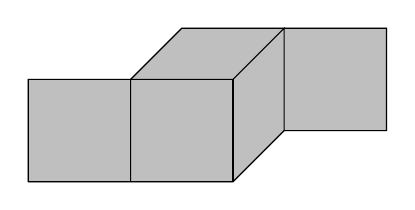
\begin{tikzpicture}[scale=1.3]
	\draw[fill,color=lightgray] (0,0) -- (1,0) -- (2,0) -- (2.5,0.5) -- (3.5,0.5) -- (3.5,1.5) -- (2.5,1.5) -- (1.5,1.5) -- (1,1) -- (0,1) -- (0,0);
	\draw (0,0) -- (1,0) -- (2,0) -- (2.5,0.5) -- (3.5,0.5) -- (3.5,1.5) -- (2.5,1.5) -- (1.5,1.5) -- (1,1) -- (0,1) -- (0,0);
	\draw (1,0) -- (1,1) -- (2,1) -- (2.5,1.5) -- (2.5,0.5);
	\draw (2,0) -- (2,1);
	\end{tikzpicture} \hspace{2cm}
	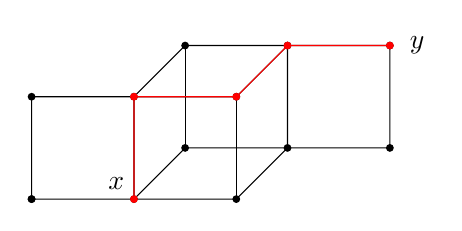
\begin{tikzpicture}[scale=1.3]
	\draw (0,0) node[fill,circle,inner sep=1pt]{} -- (1,0) node[fill,circle,inner sep=1pt]{} -- (2,0) node[fill,circle,inner sep=1pt]{} -- (2.5,0.5) node[fill,circle,inner sep=1pt]{} -- (3.5,0.5) node[fill,circle,inner sep=1pt]{} -- (3.5,1.5) node[fill,circle,inner sep=1pt]{} -- (2.5,1.5) node[fill,circle,inner sep=1pt]{} -- (1.5,1.5) node[fill,circle,inner sep=1pt]{} -- (1,1) node[fill,circle,inner sep=1pt]{} -- (0,1) node[fill,circle,inner sep=1pt]{} -- (0,0) node[fill,circle,inner sep=1pt]{};
	\draw (1,0) -- (1,1) -- (2,1) node[fill,circle,inner sep=1pt]{} -- (2.5,1.5) -- (2.5,0.5) -- (1.5,0.5) node[fill,circle,inner sep=1pt]{} -- (1,0);
	\draw (2,0) -- (2,1) ;
	\draw (1.5,0.5) -- (1.5,1.5);
	
	\draw[color=red] (1,0) node[fill,circle,inner sep=1pt]{} -- (1,1) node[fill,circle,inner sep=1pt]{} -- (2,1) node[fill,circle,inner sep=1pt]{} -- (2.5,1.5) node[fill,circle,inner sep=1pt]{} -- (3.5,1.5) node[fill,circle,inner sep=1pt]{};
	
	\draw (1,0) node[anchor=south east] {$x$};
	\draw (3.6,1.5) node[right] {$y$};
	\end{tikzpicture}
	\caption{Ein kubischer Komplex und sein $1$-Skelett. Es gilt $D(x,y) = 4$.} 
\end{figure}

\begin{bemerkung}
	Offensichtlich ist $D$ eine Metrik, da $D$ mit der Längenmetrik auf dem kubischen Komplex $X^{(1)}$ (eingeschränkt auf $X^{(0)}$) übereinstimmt. Insbesondere gilt $d_\ell(x,y) \leq D(x,y)$ für alle $x,y \in X^{(0)}$, da jeder Weg in $X^{(1)}$ auch ein Weg in $X$ ist.
\end{bemerkung}

\begin{definition}[Hyperebenen in kubischen Komplexen]
	Sei $X$ ein kubischer Komplex. Betrachte die durch
	\[ e \parallel e' \quad :\Leftrightarrow \quad e \text{ liegt gegenüber } e' \text{ in einem } 2\text{-Würfel von } X\]
	erzeugte Äquivalenzrelation auf der Menge der Kanten ($1$-Würfel) von $X$. Zwei Kanten $e, e'$ heißen \textbf{quadratäquivalent}, wenn $e \parallel e'$ gilt. \\	
	Der $i$-te \textbf{Mittelwürfel} von $C := [0,1]^n$ für $1 \leq i \leq n$ ist gegeben durch
	\[
	M_i := \penbrace*{x \in C : x_i = \frac{1}{2}} = [0,1]^{i-1} \times \penbrace*{\frac{1}{2}} \times [0,1]^{n-i}.
	\]
	Ein Mittelwürfel $M$ in $X$ heißt \textbf{transversal} zu $e$, wenn $M \cap X^{(1)}$ aus Mittelpunkten von zu $e$ quadratäquivalenten Kanten besteht. In diesem Fall schreiben wir $M \pitchfork e$. \\
	Die Vereinigung $H(e)$ aller zu $e$ transversalen Mittelwürfel heißt \textbf{Hyperebene} zu $e$.
	\[ H(e) := \bigcup_{M \pitchfork e} M \]
\end{definition}
Eine Hyperebene $H$ in einem vollständigen $\cat$ kubischen Komplex $X$ partitioniert $X$ in die drei disjunkten Teilmengen $H, U^+$ und $U^-$, wie im Bild unten zu sehen ist (vgl. auch \cite[Prop. 3.4]{Schwer} und \cite[Prop. 4.10]{Sageev}). $U^+$ und $U^-$ bezeichnen wir als \textbf{Halbräume} zu $H$.

\begin{figure}[h]
	\centering
	\begin{tikzpicture}[scale=1.5]
	\draw (2,2) -- (0,2) -- (0,1) -- (2,1) -- (2,0) -- (1,0) -- (1,2) -- (1.5,2.5) -- (3.5,2.5) -- (3.5,1.5) -- (2.5,1.5) -- (2,1) -- (2,2) -- (2.5,2.5) -- (2.5,1.5);
	\draw [dashed] (1,1) -- (1.5,1.5) -- (2.5,1.5);
	\draw [dashed,color=red,ultra thick] (1.5,1.5) -- (1.5,2.5);
	\draw [color=red, very thick] (2,1) -- (2,2);
	\draw [color=red, very thick] (1,1) -- (1,2);
	\draw [color=red, very thick] (0,1) -- (0,2);
	\draw [color=red, very thick] (2.5,1.5) -- (2.5,2.5);
	\draw [color=red, very thick] (3.5,1.5) -- (3.5,2.5);
	\draw [color=red] (2,1) node[anchor=north west]{$e$};
	
	\draw [color=blue, very thick] (0,1.5) -- (1,1.5);
	\draw [color=blue, schraffiert=blue, very thick] (1,1.5) -- (2,1.5) -- (2.5,2) -- (1.5,2) -- (1,1.5);
	\draw [color=blue, very thick] (2.5,2) -- (3.5,2);
	
	\draw [color=blue] (.5,1.5) node[below] {$H_1$};
	\draw [color=blue] (1.5,1.5) node[below] {$H_2$};
	\draw [color=blue] (3,2) node[below] {$H_3$};
	\end{tikzpicture} \hspace{2cm}
	\begin{tikzpicture}[scale=1.5]
	\draw [color=teal,schraffiert = teal] (0,1.5) -- (0,2) -- (1,2) -- (1.5,2.5) -- (3.5,2.5) -- (3.5,2) -- (2.5,2) -- (2,1.5) -- (0,1.5);
	\draw [color=orange,schraffiert = orange] (0,1) -- (1,1) -- (1,0) -- (2,0) -- (2,1) -- (2.5,1.5) -- (3.5,1.5) -- (3.5,2) -- (2.5,2) -- (2,1.5) -- (0,1.5) -- (0,1);
	\draw [color=blue, ultra thick] (0,1.5) -- (2,1.5) -- (2.5,2) -- (3.5,2);
	
	\draw [thick] (2,2) -- (0,2) -- (0,1) -- (2,1) -- (2,0) -- (1,0) -- (1,2) -- (1.5,2.5) -- (3.5,2.5) -- (3.5,1.5) -- (2.5,1.5) -- (2,1) -- (2,2) -- (2.5,2.5) -- (2.5,1.5);
	
	\draw [color=teal] (0.5,2.05) node[above] {$U^+$};
	\draw [color=orange] (2.05,.5) node[right] {$U^-$};
	\draw [color=blue] (3.55,2) node[right] {$H(e)$};
	\end{tikzpicture}
	\caption[caption]{Die Hyperebene zu $e$ ist gegeben durch $H(e) = H_1 \cup H_2 \cup H_3$.\\\hspace{\textwidth} Es gilt $X = U^+ \cup H(e) \cup U^-$.}
\end{figure}

\begin{beispiel}
	\mbox{} \\[-1.4cm]
\begin{itemize}
	\item In einem Baum sind Mittelwürfel gerade die Mittelpunkte der Kanten. Da in einem Baum keine $2$-Würfel existieren, gibt es zu einer Kante $e$ keine weiteren quadratäquivalenten Kanten. Demzufolge ist der Mittelpunkt von $e$ die Hyperebene zu $e$.
	\item Im $\RR^n$ sind die Hyperebenen achsenparallele Ebenen der Kodimension $1$, also affine Untervektorräume der Form $H_{i,k} = \{(x_1,\dots,x_n) \in \RR^n : x_i = k - 0.5\}$ mit $1 \leq i \leq n$ und $k \in \ZZ$.
	\begin{figure}[h]
		\centering
		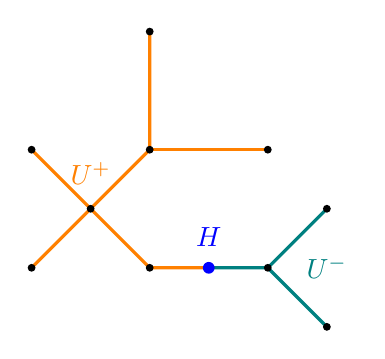
\begin{tikzpicture}[scale=1.5]
		\draw [very thick,color=orange] (0,0) -- (.5,.5) -- (1,0) -- (1.5,0);
		\draw [very thick,color=orange] (0,1) -- (.5,.5) -- (1,1) -- (1,2);
		\draw [very thick,color=orange] (1,1) -- (2,1);
		\draw [color=orange] (0.5,0.8) node{$U^+$};
		
		\draw [very thick,color=teal] (1.5,0) -- (2,0) -- (2.5,0.5);
		\draw [very thick,color=teal] (2,0) -- (2.5,-0.5);
		\draw [color=teal] (2.5,0) node{$U^-$};
		
		\draw (0,0) node[fill,circle,inner sep=1pt]{};
		\draw (.5,.5) node[fill,circle,inner sep=1pt]{};
		\draw (0,1) node[fill,circle,inner sep=1pt]{};
		\draw (1,1) node[fill,circle,inner sep=1pt]{};
		\draw (1,2) node[fill,circle,inner sep=1pt]{};
		\draw (2,1) node[fill,circle,inner sep=1pt]{};
		\draw (1,0) node[fill,circle,inner sep=1pt]{};
		\draw (2,0) node[fill,circle,inner sep=1pt]{};
		\draw (2.5,-.5) node[fill,circle,inner sep=1pt]{};
		\draw (2.5,.5) node[fill,circle,inner sep=1pt]{};
		
		\draw [color=blue] (1.5,0) node[fill,circle,inner sep=1.5pt]{};
		\draw [color=blue] (1.5,0.1) node[above]{$H$};
		\end{tikzpicture} \hspace{2cm}
		\begin{tikzpicture}[scale=0.8]
		\path [schraffiert=teal] (-1.5,-1.5) rectangle (1.5,3.5);
		\path [schraffiert=orange] (1.5,3.5) rectangle (3.5,-1.5);
		
		\draw [color=teal] (-.5,-1.5) node[below]{$U^-$};
		\draw [color=orange] (3,-1.5) node[below]{$U^+$};
		
		\draw [->,ultra thick] (-1.5,0) -- (4,0) node[right]{$x_1$};
		\draw [->,ultra thick] (0,-1.5) -- (0,4) node[right]{$x_2$};
		\foreach \x in {-1,1,2,3} {
			\draw (-1.5,\x) -- (3.5,\x);
			\draw (\x,-1.5) -- (\x,3.5);
		}
		
		\foreach \x in {-1,0,...,3} {
			\draw [ultra thick, color=red] (1,\x) -- (2,\x);
		}
		
		\draw [color=red] (2,1) node[anchor=north west]{$e$};
		
		\draw [color=blue,ultra thick] (1.5,3.5) -- (1.5,-1.5) node[below] {$H_{1,2}$};
		\end{tikzpicture}
		\caption{Beispiele für Hyperebenen in Bäumen und im $\RR^2$.}
	\end{figure}
\end{itemize}
\end{beispiel}

\section{Eigenschaft (FC)}
\label{sec:property_FC}
	In diesem Abschnitt möchten wir auf das von \textsc{Niblo} und \textsc{Reeves} formulierte Resultat über Gruppenwirkungen von Gruppen mit Eigenschaft $\prT$ auf vollständige $\cat$ kubische Komplexe eingehen. Wir orientieren uns dabei an dem Vorgehen in \cite{NibloReeves}, wofür wir unter anderem den Begriff des bedingt negativen Kerns und eine weitere äquivalente Charakterisierung der Eigenschaft $\prT$ verwenden.
	
\begin{definition}[Zelluläre Gruppenwirkung]
	Seien $X, Y$ zwei kubische Komplexe. Eine Abbildung $\varphi \colon X \rightarrow Y$ heißt \textbf{zellulär}, wenn für jeden Würfel $C \subseteq X$ mit $\dim(C) = n$ das Bild $\varphi(C)$ ein Würfel in $Y$ ist mit $\dim(\varphi(C)) \leq n$. \\
	Eine Gruppenwirkung $\Phi \colon G \rightarrow \Isom(X)$ einer Gruppe $G$ heißt \textbf{zellulär}, wenn die Abbildung $\Phi(g)$ zellulär ist für alle $g \in G$. Insbesondere gilt dann $\Phi(g)(x_0) \in X^{(0)}$ für alle $x_0 \in X^{(0)}$.
\end{definition}
\newpage
\begin{definition}[Eigenschaft $\prFC$]
	Eine Gruppe $G$ hat \textbf{Eigenschaft (FC)}, wenn jede zelluläre Wirkung $\Phi \colon G \rightarrow \Isom(X)$ von $G$ auf einen vollständigen $\cat$ kubischen Komplex $X$ einen globalen Fixpunkt besitzt.
\end{definition}

\begin{definition}[bedingt negativ definiter Kern]
\label{def_cnk}
	Sei $X$ eine Menge. Ein \textbf{bedingt negativ definiter Kern} auf $X$ ist eine Abbildung $f \colon X \times X \rightarrow \RR$ mit folgenden Eigenschaften:
	\begin{enumerate}[(1)]
		\item Für alle $x \in X$ ist $f(x,x) = 0$.
		\item Für alle $x,y \in X$ ist $f(x,y) = f(y,x)$.
		\item Für jede endliche Teilmenge $\{x_1,\dots,x_n\} \subseteq X$ und $\lambda_1, \dots, \lambda_n \in \RR$ mit $\sum_{i=1}^{n} \lambda_i = 0$ gilt
		\[ \sum_{1 \leq i,j \leq n} \lambda_i \lambda_j f(x_i,x_j) \leq 0\]
	\end{enumerate}
	Ein bedingt negativ definiter Kern $f$ auf einer Gruppe $G$ ist zusätzlich linksinvariant, das heißt er erfüllt die folgende Eigenschaft:
	\begin{enumerate}[(1)] \setcounter{enumi}{3}
		\item Für alle $g,h,k \in G$ gilt $f(gh,gk) = f(h,k)$.
	\end{enumerate}
\end{definition}

\begin{satz}[{\cite[Theorem 2.10.4]{BekkaHarpeValette}}]
	Sei $G$ eine endlich erzeugte Gruppe. $G$ hat genau dann die Eigenschaft $\prT$, wenn jeder bedingt negativ definite Kern auf $G$ beschränkt ist.
\end{satz}

Die Aussage ist in \cite{BekkaHarpeValette} ursprünglich für allgemeine topologische Gruppen und die Eigenschaft $\prFH$ anstelle der Eigenschaft $\prT$ formuliert. Zusammen mit Theorem~\ref{thm:kap2} folgt aber die für uns relevante Aussage über die von uns betrachteten endlich erzeugten Gruppen.

Sei nun $(X,d_\ell)$ ein vollständiger $\cat$ kubischer Komplex und $G$ eine endlich erzeugte Gruppe, die zellulär auf $X$ wirkt. Wir halten nun einige Eigenschaften der simplizialen Metrik fest, die wir für den Beweis des Hauptresultats dieses Kapitels benötigen.

\begin{lemma}[Eigenschaften der simplizialen Metrik]
	\label{lemma_simp_metr} \mbox{} \\[-1.4cm]
	\begin{enumerate}[(i)]
		\item Es gilt $D(x,y) = \sum\limits_{U} \chi_U(x) \cdot (1 - \chi_U(y))$, wobei $U$ über alle Halbräume von $X$ läuft und $\chi_U$ die charakteristische Funktion von $U$ ist.
		\item $D$ ist ein bedingt negativ definiter Kern auf $X^{(0)}$.
		\item $D$ ist invariant bezüglich jeder Wirkung $\Phi$ von $G$ auf $X^{(0)}$, das heißt
		\[D(\Phi(g)(x),\Phi(g)(y)) = D(x,y) \quad \forall g \in G, x,y \in X^{(0)} \]
	\end{enumerate}
\end{lemma}

\begin{beweis}[{vgl. \cite[Technical Lemma]{NibloReeves}}]
	\mbox{} \\[-.85cm]
	\begin{enumerate}[(i)]
		\item Seien $x,y \in X^{(0)}$ beliebig. \textsc{Sageev} hat in \cite{Sageev} gezeigt, dass jeder kürzeste Weg $\sigma$ von $x$ nach $y$ in $X^{(1)}$ jede Hyperebene von $X$ höchstens einmal schneidet. Da die geschnittenen Hyperebenen gerade aus Mittelwürfeln bestehen, die transversal zu den zu $\sigma$ gehörenden Kanten sind, folgt, dass jede Kante von $\sigma$ genau eine Hyperebene schneidet. Demzufolge ist die Länge von $\sigma$ gegeben durch die endliche Anzahl an Hyperebenen zwischen $x$ und $y$. Diese Hyperebenen liefern genau diejenigen Halbräume von $X$ die entweder $x$ oder $y$ enthalten ($x$ und $y$ liegen nicht auf einer Hyperebene, da diese die Kanten nur in ihren Mittelpunkten schneiden und nicht in Punkten aus $X^{(0)}$). Jede Hyperebene liefert zwei Halbräume: Einen Halbraum $U^+ \subseteq X$ mit $x \in U^+, y \notin U^+$, und einen Halbraum $U^- \subseteq X$ mit $x \notin U^-, y \in U^-$.
		
		\begin{figure}[h]
			\centering
			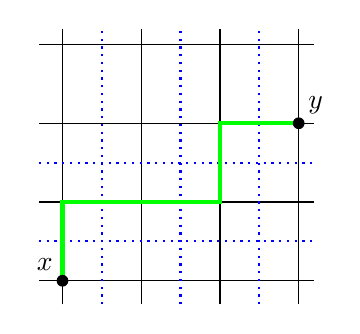
\begin{tikzpicture}[scale=1]
			\foreach \x in {1,...,4} {
				\draw (\x,0.7) -- (\x,4.2);
				\draw (0.7,\x) -- (4.2,\x);
			}
			
			\foreach \x in {1,2} {
				\draw [color=blue,dotted,thick] (0.7,\x+.5) -- (4.2,\x +.5);
				\draw [color=blue,dotted,thick] (\x+.5,0.7) -- (\x+.5,4.2);
			}
			
			\draw [color=blue,dotted,thick] (3.5,0.7) -- (3.5,4.2);
			
			\draw [color=green,ultra thick] (1,1) -- (1,2) -- (3,2) -- (3,3) -- (4,3);
			
			\draw (1,1) node[fill,circle,inner sep=1.5pt]{};
			\draw (4,3) node[fill,circle,inner sep=1.5pt]{};
			\draw (1,1) node[anchor=south east]{$x$};
			\draw (4,3) node[anchor=south west]{$y$};
			\end{tikzpicture} \hspace{2cm}
			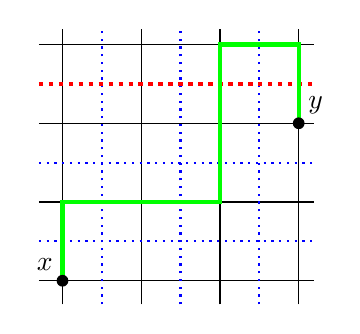
\begin{tikzpicture}[scale=1]
			\foreach \x in {1,...,4} {
				\draw (\x,0.7) -- (\x,4.2);
				\draw (0.7,\x) -- (4.2,\x);
			}
			
			\foreach \x in {1,2} {
				\draw [color=blue,dotted,thick] (0.7,\x+.5) -- (4.2,\x +.5);
				\draw [color=blue,dotted,thick] (\x+.5,0.7) -- (\x+.5,4.2);
			}
			
			\draw [color=blue,dotted,thick] (3.5,0.7) -- (3.5,4.2);
			\draw [color=red,dotted,ultra thick] (.7,3.5) -- (4.2,3.5);
			
			\draw [color=green,ultra thick] (1,1) -- (1,2) -- (3,2) -- (3,4) -- (4,4) -- (4,3);
			
			\draw (1,1) node[fill,circle,inner sep=1.5pt]{};
			\draw (4,3) node[fill,circle,inner sep=1.5pt]{};
			\draw (1,1) node[anchor=south east]{$x$};
			\draw (4,3) node[anchor=south west]{$y$};
			\end{tikzpicture}
			\caption{Links: Ein kürzester Weg zwischen $x$ und $y$. Rechts: Ein längerer Weg, der eine Hyperebene zwei Mal schneidet.}
		\end{figure}
		
		Somit stimmt die Anzahl der Hyperebenen zwischen $x$ und $y$ überein mit der Anzahl der Halbräume von $X$, die $x$ enthalten und $y$ nicht. Zusammengefasst:
		\begin{equation}
		\begin{aligned}
		D(x,y) &= \inf \{ \ell(\sigma) : \sigma \text{ ist Weg von } x \text{ nach } y \text{ in } X^{(1)}\} \\
		&= \#\{H \subseteq X : H \text{ ist Hyperebene zwischen } x \text{ und } y\} \\
		&= \#\{U \subseteq X \text{ Halbraum} : x \in U, y \notin U \} \\
		&= \sum_{\substack{U \subseteq X \\ \text{Halbraum}}} \underbrace{\chi_U(x) \cdot (1- \chi_U(y))}_{= 1 \Leftrightarrow x \in U \wedge y \notin U}
		\end{aligned}
		\end{equation}
		\item Zu zeigen sind die Eigenschaften (1), (2) und (3) aus Definition \ref{def_cnk}. \\
		(1) und (2) sind klarerweise erfüllt, da $D$ eine Metrik ist. Sei also $V:= \{x_1, \dots, x_n\} \subseteq X^{(0)}$ endlich sowie $\lambda_1, \dots, \lambda_n \in \RR$ mit $\sum_{i=1}^{n} \lambda_i = 0$. Dann ist
		\[ \sum\limits_{1 \leq i,j \leq n} \lambda_i \lambda_j D(x_i,x_j) = \sum\limits_{i=1}^{n} \sum\limits_{j=1}^{n} \lambda_i \lambda_j \sum\limits_{U} \chi_U (x_i) (1-\chi_U (x_j))\]
		\newpage
		Da für jedes Paar $(x_i,x_j) \in V \times V$ höchstens endlich viele Hyperebenen zwischen $x_i$ und $x_j$ verlaufen, existieren insgesamt nur endlich viele Halbräume $U \subseteq X$, für die der Ausdruck\linebreak $\chi_U(x_i) \cdot (1-\chi_U(x_j))$ in der hinteren Summe nicht verschwindet. Insbesondere ist die hintere Summe endlich. Bezeichnen wir jene Halbräume mit $U_1, \dots, U_m$, ermöglicht dies folgende Umformungen:
		
		\begin{equation}
		\begin{aligned}
		\ &\sum\limits_{i=1}^{n} \sum\limits_{j=1}^{n} \lambda_i \lambda_j \sum\limits_{k=1}^m \chi_{U_k} (x_i) - \sum\limits_{i=1}^{n} \sum\limits_{j=1}^{n} \lambda_i \lambda_j \sum\limits_{k=1}^m \chi_{U_k} (x_i) \cdot \chi_{U_k} (x_j) \\
		= \  &\underbrace{\sum\limits_{j=1}^{n} \lambda_j}_{=0} \sum\limits_{i=1}^{n} \lambda_i \sum\limits_{k=1}^m \chi_{U_k} (x_i) - \sum\limits_{k=1}^m \sum\limits_{i=1}^{n} \lambda_i \chi_{U_k}(x_i) \sum\limits_{j=1}^{n} \lambda_j \chi_{U_k} (x_j) \\
		= \ &0 - \sum\limits_{k=1}^m \enbrace*{\sum\limits_{i=1}^n \lambda_i \chi_{U_k} (x_i)}^2 
		\leq 0
		\end{aligned}
		\end{equation}
		\item Wie oben zur Definition bemerkt, stimmt die simpliziale Metrik $D$ auf $X^{(0)}$ mit der Längenmetrik $d_{X^{(1)}}$ von $X^{(1)}$ eingeschränkt auf $X^{(0)}$ überein. Da $(X^{(1)},d_{X^{(1)}})$ ein kubischer Komplex ist, vermittelt $\Phi$ auch eine zelluläre (und damit isometrische) Wirkung $\widetilde{\Phi}$ auf $X^{(1)}$ vermöge $\widetilde{\Phi}(g) := \Phi(g) \big|_{X^{(1)}}$, das heißt für alle $x,y \in X^{(0)} \subseteq X^{(1)}$ und $g \in G$ gilt
		\[ D(\Phi(g)(x),\Phi(g)(y)) = d_{X^{(1)}}(\widetilde{\Phi}(g)(x),\widetilde{\Phi}(g)(y)) = d_{X^{(1)}}(x,y) = D(x,y) \qedhere \]		
	\end{enumerate}
\end{beweis}

Bevor wir zum Theorem kommen, das diesen Abschnitt abschließt, erwähnen wir ein Resultat von \textsc{Gerasimov}. Dieses ist ein Korollar aus dem \textsc{Bruhat-Tits}-Fixpunktsatz und wird uns im folgenden Beweis die Existenz eines Fixpunktes liefern.

\begin{satz}[Gerasimov {\cite[Lemma 5.18]{Cornulier}}]
\label{satz:gerasimov}
	Sei $\Phi\colon G \rightarrow \Isom(X)$ eine zelluläre Wirkung einer Gruppe $G$ auf einen $\cat$ kubischen Komplex $X$. Existiert ein $x \in X$ mit beschränktem Orbit, so hat $\Phi$ einen globalen Fixpunkt.
\end{satz}

\begin{theo}
\label{thm:kap3}
	Sei $X$ ein vollständiger $\cat$ kubischer Komplex und $G$ eine endlich erzeugte Gruppe, die die Kazhdan-Eigenschaft $\prT$ erfüllt. Dann hat jede zelluläre Wirkung von $G$ auf $X$ einen globalen Fixpunkt. Mit anderen Worten:
	Besitzt $G$ die Eigenschaft $\prT$, dann ebenfalls die Eigenschaft $\prFC$.
\end{theo}
\newpage
\begin{beweis}[vgl. {\cite[Theorem B]{NibloReeves}}]
	Sei $\Phi\colon G \rightarrow \Isom(X)$ eine beliebige zelluläre Wirkung von $G$ auf $X$. Dann ist $\Phi\big|_{X^{(0)}}\colon G \rightarrow \Isom(X^{(0)})$ eine zelluläre Wirkung auf dem $0$-Skelett von $X$. Wir fixieren ein $v \in X^{(0)}$ beliebig und betrachten die Abbildung
	\begin{equation}
	\begin{aligned}
	f_v\colon G \times G &\longrightarrow \RR \\
	(g,h) &\longmapsto D(\Phi(g)(v),\Phi(h)(v))
	\end{aligned}
	\end{equation}
	Wir zeigen, dass $f_v$ ein bedingt negativ definiter Kern auf $G$ ist. Die Eigenschaften (1), (2) und (3) sind klarerweise erfüllt, da $D$ ein bedingt negativ definiter Kern ist. Die Linksinvarianz von $f_v$ folgt aus der Invarianz von $D$: Für beliebige $g,h,k \in G$ gilt:
	\begin{equation}
	\begin{aligned}
	f_v(gh,gk) &= D(\Phi(gh)(v),\Phi(gk)(v)) \\
	&= D(\Phi(g)(\Phi(h)(v)),\Phi(g)(\Phi(k)(v))) \\
	&= D(\Phi(h)(v),\Phi(k)(v)) \\
	&= f_v(h,k)
	\end{aligned}
	\end{equation}
	Die Gruppe $G$ hat Eigenschaft $\prT$, also ist $f_v$ beschränkt, das heißt die Menge
	$f_v(G \times G) = D(\Phi(G)(v) \times \Phi(G)(v))$ ist beschränkt in $\RR$. Damit ist der Orbit $\Phi(G)(v)$ von $v$ beschränkt bezüglich $D$ und wegen $d_\ell \leq D$ auch bezüglich $d_\ell$. Nach Voraussetzung ist $(X,d_\ell)$ $\cat$. Nach Satz~\ref{satz:gerasimov} folgt somit die Existenz eines globalen Fixpunktes.
\end{beweis}

Aus dem Theorem folgt unmittelbar, dass jede Gruppe mit Kazhdan-Eigenschaft $\prT$ eine weitere Fixpunkteigenschaft besitzt: Da simpliziale Bäume ebenfalls vollständige $\cat$ kubische Komplexe sind, folgt aus der Eigenschaft $\prT$ somit auch die von \textsc{Serre} formulierte Eigenschaft $\prFA$:

\begin{korollar}[Eigenschaft $\prFA$]
	Sei $G$ eine endlich erzeugte Gruppe, die die Eigenschaft $\prT$ besitzt. Dann besitzt $G$ auch die Eigenschaft $\prFA$, das heißt jede zelluläre Wirkung von $G$ auf einen simplizialen Baum besitzt einen globalen Fixpunkt (in der geometrischen Realisierung).
\end{korollar}

\cleardoubleoddemptypage